\documentclass{article}
\usepackage{enumitem} % Para listas personalizadas
\usepackage{graphicx} % Required for inserting images
\usepackage{hyperref}


\title{Aplicaciones de la IA en los videojuegos y expectativas futuras}
\author{Rommel Antonio Cedeño López}
\date{September 2024}

\begin{document}

\maketitle

\begin{abstract}
    La inteligencia artificial (IA) ha sido aplicada en la industria de los videojuegos, impulsando mejoras significativas en la experiencia de juego. El artículo analiza varios algoritmos de IA utilizados para optimizar el contenido de los juegos, basándose en los intereses de los jugadores. Además, evalúa cómo la IA ha perfeccionado las interacciones entre los jugadores y los elementos del juego, creando experiencias más inmersivas.
\\

El artículo también explora las expectativas futuras de la IA en los videojuegos, tanto en términos de optimización de experiencias como en mejoras visuales y de hardware. Concluye destacando los beneficios potenciales del uso continuo de algoritmos de IA para el desarrollo de videojuegos.
\end{abstract}


\section{Introduction}
La inteligencia artificial (IA) aplicada a los videojuegos permite recrear comportamientos humanos, analizando y respondiendo a diversas situaciones dentro del juego. Desde sus inicios en los juegos de mesa, donde se utilizaba para calcular estrategias, hasta su expansión en géneros como disparos, aventuras y juegos de rol, la IA ha evolucionado hacia modelos más humanos que simulan emociones y comportamientos. Esta tecnología busca ofrecer una experiencia realista mediante interacciones visuales y reacciones de los personajes dentro del juego, aunque aún necesita mejoras para alcanzar un mayor realismo.
\\

Uno de los principales retos de la IA en videojuegos radica en los defectos de los modelos de entrenamiento y los altos costos técnicos que enfrentan las empresas. El artículo proporciona una visión general de los conceptos de IA en la industria del videojuego, destacando cómo esta tecnología ha mejorado la jugabilidad y explorando los tipos de algoritmos utilizados. Además, ofrece una referencia para futuros desarrollos en este campo, subrayando el impacto de la IA en el crecimiento de este mercado.



\subsection{Algoritmos de IA aplicados en videojuegos:
}
Se presentan cinco algoritmos de IA usados en juegos: aprendizaje por refuerzo, aprendizaje por imitación, máquina de estados finitos (FSM), máquina de estados difusos (FuSM) y algoritmo genético (GA). Estos modelan los comportamientos de los sistemas de manera diversa.

\subsection{Aprendizaje  por  refuerzo}
El aprendizaje por refuerzo permite a los agentes en videojuegos tomar decisiones basadas en el entorno utilizando el Proceso de Decisión de Markov (MDP), que incluye estados, acciones, recompensas y una política. Los agentes observan el estado actual, eligen acciones y reciben retroalimentación en forma de recompensas o castigos, lo que ajusta sus futuras decisiones para maximizar beneficios a largo plazo. La política, que guía las acciones del agente, se optimiza iterativamente a través de este sistema de retroalimentación, mejorando el comportamiento del agente a medida que aprende de sus interacciones con el entorno.
\\

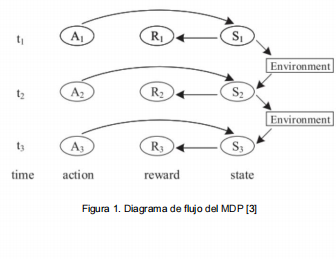
\includegraphics{MDP.png}
\\

\title{\textbf{Función}}

Dentro de los videojuegos es proporcionar una estructura matemática que permita a un agente (como un personaje o NPC) tomar decisiones óptimas de manera autónoma. El agente interactúa con el entorno del juego, seleccionando acciones que influyen en su estado, mientras maximiza una recompensa acumulada a lo largo del tiempo.
\\

\subsection{Aprendizaje por imitación}
El aprendizaje por imitación permite a los agentes aprender estrategias a partir de demostraciones estado-acción, comúnmente en juegos. GAIL utiliza técnicas generativas adversariales para imitar expertos, optimizando acciones mediante aprendizaje de refuerzo. BC es un método supervisado que aprende de trayectorias expertas, aunque su eficiencia depende de la disponibilidad de datos. Ambos enfoques mejoran el rendimiento de agentes en juegos. La máquina de estados finitos (FSM) gestiona comportamientos y transiciones de personajes en juegos, definiendo estados como "caminar" o "atacar" según condiciones predefinidas.

\subsection{GAIL (Aprendizaje por Imitación Generativa Adversarial)}
Es una técnica de aprendizaje que busca imitar el comportamiento de un experto a través de un enfoque generativo y competitivo. Su objetivo es que un modelo aprenda a actuar de manera similar a un modelo experto, basándose en la imitación de sus acciones.
\\
\\
GAIL funciona de la siguiente manera: crea un entorno donde el agente (el personaje del juego o sistema) aprende observando a un modelo experto y luego intenta imitar sus decisiones. 

\subsection{BC (Behavior Cloning)}
BC (Behavior Cloning) es un método de aprendizaje supervisado que permite a los agentes de juego aprender a partir de trayectorias de expertos, imitando sus acciones en función del estado observado. Aunque requiere una gran cantidad de datos de ejemplo, su eficacia puede verse limitada por la falta de ejemplos adecuados y la dificultad de obtener datos relevantes. En el contexto de los juegos, BC se utiliza para entrenar agentes mediante la imitación, mientras que GAIL se enfoca en reducir la brecha de rendimiento entre el agente y el experto, mejorando así la experiencia de juego al entrenar agentes más inteligentes.

\subsection{FSM}

La máquina de estados finitos (FSM) es un modelo matemático ampliamente utilizado en el desarrollo de videojuegos para gestionar el comportamiento de personajes y objetos. Funciona a través de un conjunto limitado de estados, como "caminar", "inactivo" o "atacar", y reglas que definen las transiciones entre estos estados. En los juegos, cada personaje u objeto se puede representar como una FSM, donde el estado actual y las condiciones de entrada determinan el próximo estado. Las transiciones entre estados se producen mediante eventos o condiciones específicas que activan el cambio.
\\

Los principios de aplicación de FSM en juegos son los siguientes:
\begin{itemize}
    \item \textbf{Estado:} Representa los comportamientos o situaciones de un objeto en el juego, como "caminar" o "atacar", con atributos específicos.
    \item \textbf{Condición de transición:} Son eventos que activan el cambio de un estado a otro, como pasar de "inactivo" a "herido" tras un ataque.
    \item \textbf{Acción:} Son las tareas que el FSM realiza en cada estado, como ajustar la velocidad y dirección cuando un personaje está "caminando."
    \item \textbf{Gráfico de transición:} Es la representación visual del FSM, mostrando estados y las transiciones entre ellos, facilitando la gestión de comportamientos.
\end{itemize}

Las FSM simplifican la gestión de la lógica del juego y permiten mayor control y flexibilidad.

\subsection{FuSM} 
FuSM (Fuzzy State Machine) y el algoritmo de lógica difusa son técnicas utilizadas en el desarrollo de juegos para implementar comportamientos inteligentes en NPCs, proporcionando una mayor flexibilidad frente a las máquinas de estados tradicionales (FSM). A diferencia de las FSM, que funcionan con estados discretos y transiciones deterministas, las FuSM permiten la superposición de estados, utilizando lógica difusa para realizar transiciones más suaves y graduales entre ellos. Cada estado tiene un valor difuso que determina el grado de confianza, lo que permite a los personajes adaptarse mejor a cambios en el entorno, como en un juego de combate donde las decisiones se basan en datos como salud y número de enemigos. En juegos como League of Legends, los jugadores poseen múltiples habilidades con diferentes niveles de activación, lo que hace que sus comportamientos sean menos predecibles y, por tanto, más interesantes que en los juegos basados en FSM.
\\
\\
\title{\textbf{Algoritmo de lógica difusa de IA:}}
El algoritmo de lógica difusa de IA se utiliza en juegos para la toma de decisiones de personajes, como enemigos o uso de elementos, basado en reglas y conjuntos difusos. A diferencia de la lógica booleana que maneja valores verdaderos o falsos, la lógica difusa permite grados intermedios de verdad (entre 0 y 1), lo que facilita la simulación de decisiones más complejas y parecidas al razonamiento humano. Esto lo hace ideal para enfrentar problemas como el reconocimiento de emociones humanas y la toma de decisiones en escenarios inciertos o ambiguos.

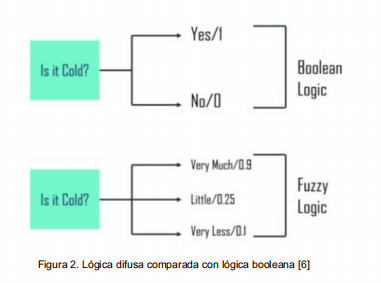
\includegraphics{Logica boolena.png}
\\

\title{\textbf{Función}}
\\
Funciona asignando grados de verdad a las decisiones en lugar de manejar respuestas estrictamente binarias (como en la lógica booleana). Mientras que la lógica booleana solo permite valores como "sí" o "no" (1 o 0), la lógica difusa admite valores intermedios entre 0 y 1. Esto permite representar decisiones con mayor flexibilidad y realismo.


\subsection{GA} 
El algoritmo genético (AG) es un método heurístico inspirado en la genética biológica que se utiliza en los videojuegos para optimizar soluciones a problemas complejos. Funciona generando una población inicial de soluciones, evaluando su aptitud según criterios específicos y seleccionando los individuos más aptos para reproducirse. A través de la combinación genética (cruce) y la mutación aleatoria, se crean nuevas soluciones que mejoran con cada generación. Este proceso se repite hasta alcanzar una solución óptima o cumplir un criterio de finalización. El AG se aplica en los juegos para optimizar el rendimiento, diseñar comportamientos inteligentes y ajustar la dificultad, proporcionando soluciones eficientes y mejorando la experiencia del jugador.
\\

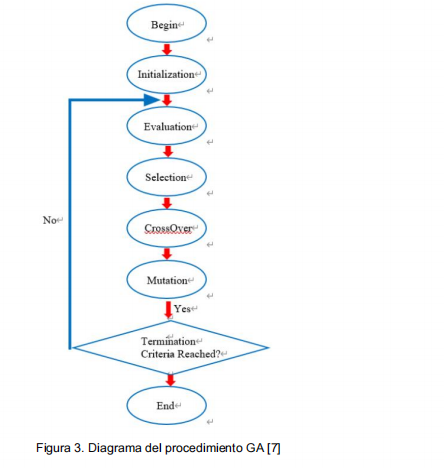
\includegraphics{GA.png}
\\
\title{\textbf{Funcion}}
\\
Su función principal en los videojuegos es encontrar soluciones óptimas a problemas complejos, como la toma de decisiones, la generación de estrategias o la adaptación de personajes a situaciones cambiantes.


\section{IA utilizada para optimizar la experiencia del jugador y el contenido del juego}

\subsection{Detección de fallos en las imágenes renderizadas}

La detección de fallos en imágenes renderizadas en videojuegos es crucial para evitar problemas gráficos que afecten la experiencia del jugador. Los DCNN (redes neuronales convolucionales profundas) se entrenan con datos, incluidas imágenes defectuosas, para reconocer patrones y detectar fallos antes de que el juego comience, lo que ayuda a prevenir errores visuales en escenas y objetos simulados.

\subsection{Equilibrio del juego}

El equilibrio del juego es fundamental para asegurar una experiencia satisfactoria al emparejar automáticamente a jugadores con niveles de habilidad similares en juegos PvP, evitando frustraciones. La IA juega un papel clave al aprender de muchas partidas, ajustando los emparejamientos para mantener desafíos adecuados. En juegos de un solo jugador, la IA también ajusta la dificultad basándose en la retroalimentación del jugador, como la pérdida de vida o muertes, garantizando una experiencia equilibrada y motivadora.

\subsection{Creación de contenidos de juego}
La IA en la creación de contenidos de juegos se utiliza para generar imágenes, textos y música de manera eficiente, entrenando modelos con datos adecuados y descripciones. Esto permite crear grandes cantidades de contenido rápidamente, reduciendo costos en el desarrollo de juegos. Además, en juegos PvP, como League of Legends, la IA puede tomar el control de un personaje si un jugador se desconecta, garantizando la continuidad del juego y evitando afectar la experiencia de los demás jugadores.

\subsection{Detección de emociones}

La detección de emociones en juegos, mediante el Modelado de Experiencia del Jugador (PEM), optimiza la experiencia al analizar el rendimiento fisiológico de los jugadores, como expresiones faciales, respiración y frecuencia cardíaca. Esto se logra con la Inteligencia Emocional Artificial (AEI), que usa sensores, cámaras y micrófonos para captar comportamientos humanos y, a través de algoritmos de aprendizaje profundo, detectar emociones como ira o miedo. Estos datos permiten ajustar la experiencia de juego según las emociones detectadas.


\subsection{Personajes no jugadores más intelectivos}
La creación de personajes no jugadores más inteligentes y realistas busca mejorar la experiencia de juego al modelar emociones y ofrecer respuestas flexibles y personalizadas. Estos personajes responden de manera única a cada jugador según sus acciones, simulando conversaciones auténticas. Herramientas como FAtiMA Toolkit permiten desarrollar personajes con inteligencia emocional, enfocándose en la naturaleza del personaje en lugar de los eventos. Además, Cif-CK ayuda a los personajes a reconocer sus propias emociones y reacciones, entrenándolos para responder adecuadamente en diversas interacciones sociales.


\subsection{Interacción con humanos}
El procesamiento del lenguaje natural (PLN) es una técnica que permite a la IA comprender y responder adecuadamente al lenguaje y comportamiento humano. En juegos PvP, por ejemplo, si un jugador envía palabras agresivas, el sistema puede imponer sanciones, como la prohibición de enviar mensajes. El análisis de sentimientos, que forma parte del PLN, clasifica las palabras en categorías como positivas o negativas, y utiliza el aprendizaje automático para entrenar modelos a partir de características de texto transformadas en vectores. Técnicas como Word Embeddings ayudan a representar las palabras en un espacio de alta dimensión, donde la distancia entre los vectores indica la similitud entre ellas.


\section{Expectativas futuras de la IA en los videojuegos}

\subsection{Más inteligencia para crear un juego}
La inteligencia artificial (IA) facilita la creación de videojuegos al permitir un desarrollo más personalizado y adaptado a las preferencias individuales de los jugadores. Mediante la predicción de gustos basados en hábitos, la IA puede recomendar elementos que se alineen con las preferencias de los usuarios, lo que ayuda a los diseñadores en el proceso de desarrollo. En juegos de mundo abierto, por ejemplo, la IA puede generar mapas personalizados que reflejen las preferencias de cada jugador. Además, una vez que el juego ha terminado, la IA puede ajustar la dificultad y la experiencia del juego para que el jugador se sienta como un experto en su próxima partida. Esto no solo reduce los costos de desarrollo, sino que también mejora la eficiencia del mismo.

\subsection{Una IA muy inteligente similar a la humana en el juego}
La inteligencia artificial (IA) en los videojuegos puede actuar como jugadores reales, imitando comportamientos humanos y ocupando el lugar de amigos o compañeros en ausencia de otros jugadores. Aunque actualmente la IA solo comprende emociones y acciones básicas, se prevé que en el futuro sea aún más similar a los humanos, aunque esto podría generar problemas morales. En pruebas de juegos, la IA puede reemplazar a los jugadores de prueba, lo que reduce costos y mejora la eficiencia y precisión en la detección de fallos, permitiendo así predecir mejores estrategias de desarrollo.

\subsection{Realidad virtual mejorada}
La realidad virtual mejorada se centra en optimizar el hardware y la interacción para crear un entorno de juego tridimensional que imite la vida real, permitiendo a los jugadores realizar acciones como volar o luchar. Este mundo virtual ofrecerá más opciones de interacción, como chatear con personajes y manipular objetos, para acercarse a la experiencia real. Aunque la realidad virtual actual es costosa y técnicamente compleja, se espera que en el futuro sea más accesible para todos los jugadores.

\subsection{Enlace a GitHub}

Visita: \url{https://github.com/Cllasd44/Inteligencia-Artificiial/blob/main/README.md}

\end{document}
